\section{Grasping Model Results}

\subsection{Top-1 Grasp Selection (Inference Indicator)}
\begin{itemize}
    \item \textbf{Dense Prediction to Single Grasp:} During inference, the model produces dense per-pixel maps for grasp quality $Q$ and grasp orientation $\theta$ (via $\cos(2\theta)$ and $\sin(2\theta)$). A practical single-grasp prediction is obtained by selecting the pixel with the maximum predicted quality (Top-1), reading the corresponding angle, and constructing a grasp rectangle centered at that pixel.
    
    \item \textbf{Post-Processing Role:} This Top-1 rule is not used as a loss term during training. Training optimizes the full dense maps, while Top-1 serves as a convenient post-processing step for visualization and for evaluating whether the highest-confidence proposal aligns with a feasible grasp.
    
    \item \textbf{Validation Metrics:} During validation, we report:
    \begin{enumerate}
        \item The validation loss.
        \item A center-angle accuracy proxy.
    \end{enumerate}    
    \item \textbf{Accuracy Proxy Definition:} The accuracy proxy selects the pixel with maximum predicted grasp quality ($\operatorname{argmax} Q$), reads the predicted angle at that pixel, and counts a sample as correct if it matches at least one positive label within a specific distance and angle threshold. This provides an intuitive indicator of whether the network's single best prediction is close to a ground-truth grasp.
\end{itemize}

% \clearpage
\subsection{Results and Comparison (ResNet-UNet vs Swin)}

Training and validation curves are used to diagnose convergence and generalization. A summary of best validation performance is presented below.

In these plots, a steadily decreasing training loss indicates successful optimization of the objective, while the validation loss reflects generalization to unseen samples. A growing gap between training and validation loss is a typical sign of overfitting; augmentation, weight decay (AdamW), and early stopping were used to mitigate this effect on the small brick dataset.

\begin{figure}[H]
    \centering
    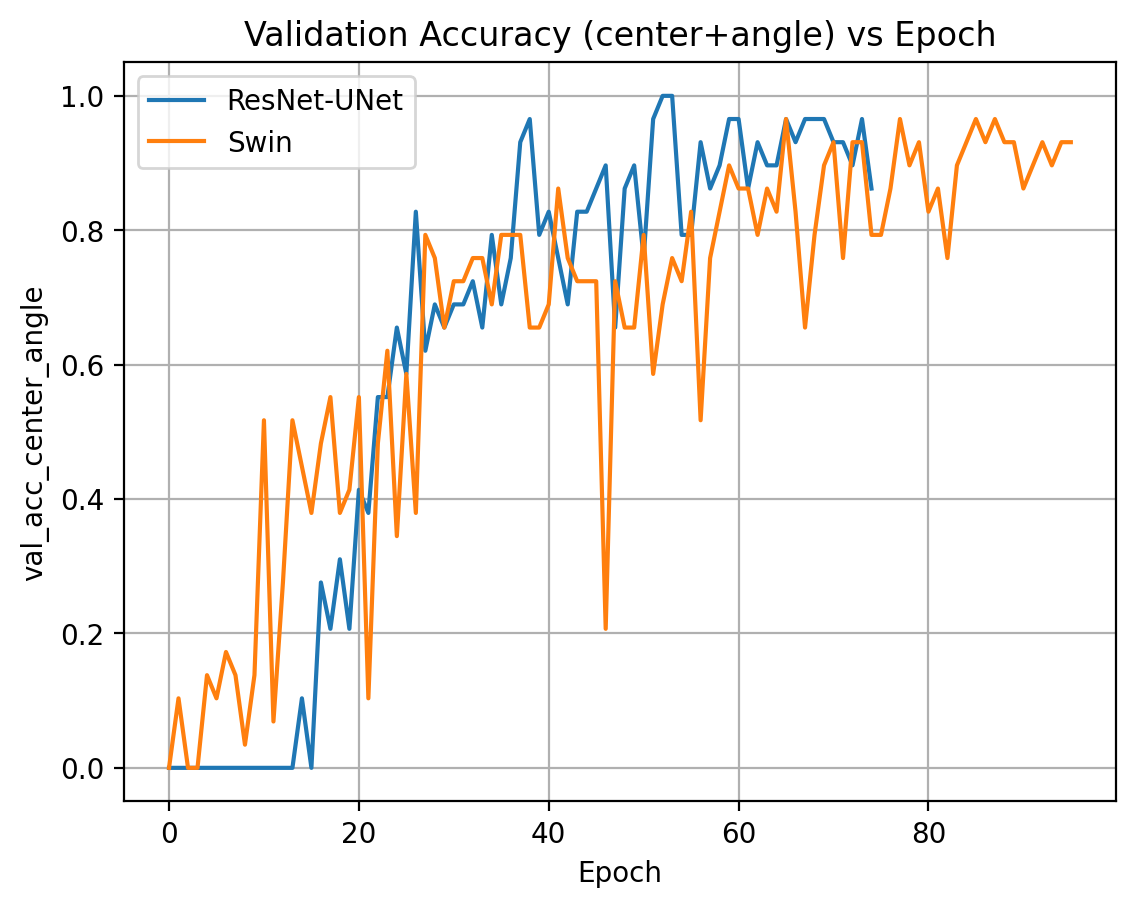
\includegraphics[width=0.7\textwidth]{Figures/chapter4/Grasping/valacc_vs_epoch.png}
    \caption{Validation loss over epochs (ResNet-UNet vs Swin).}
    \label{fig:val_loss}
\end{figure}

\begin{figure}[H]
    \centering
    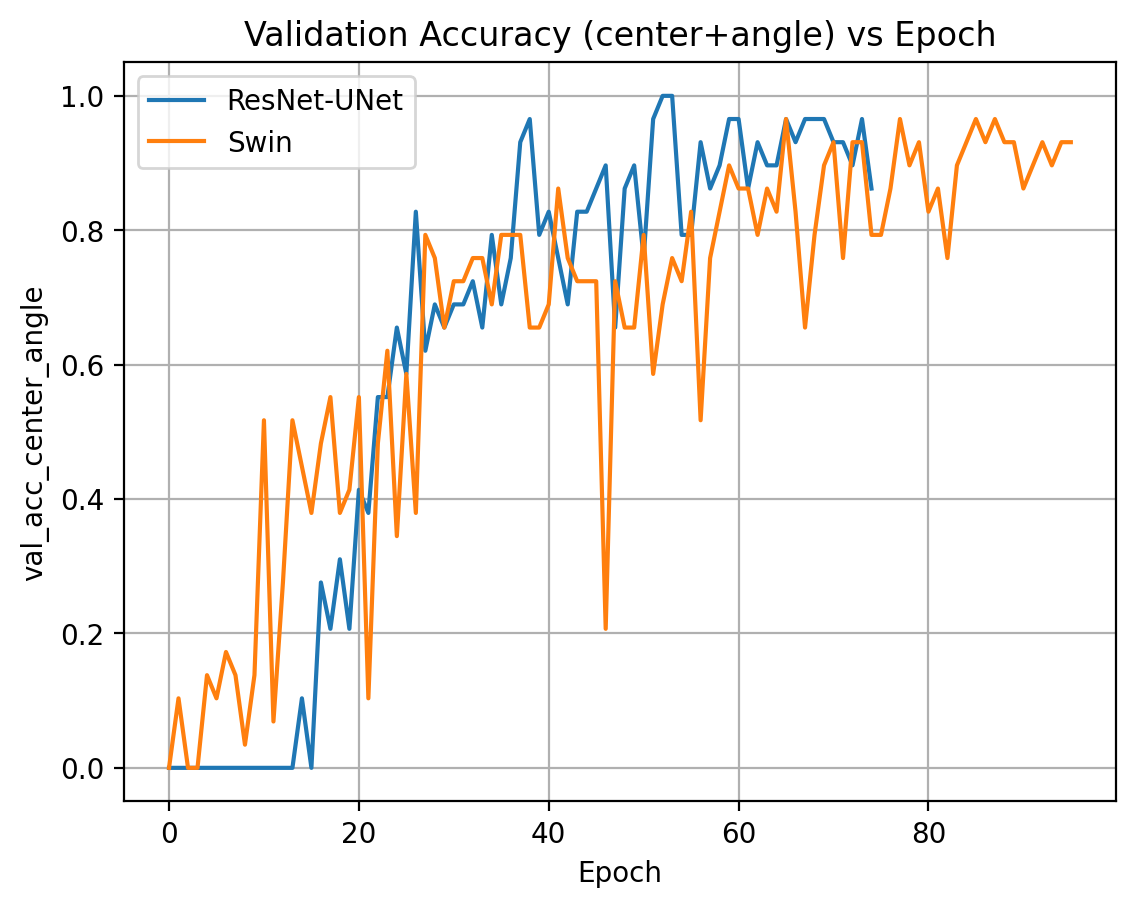
\includegraphics[width=0.6\textwidth]{Figures/chapter4/Grasping/valacc_vs_epoch.png}
    \caption{Validation best ($\operatorname{argmax}$-$Q$) center-angle accuracy over epochs (ResNet-UNet vs Swin).}
    \label{fig:val_acc}
\end{figure}

\begin{figure}[H]
    \centering
    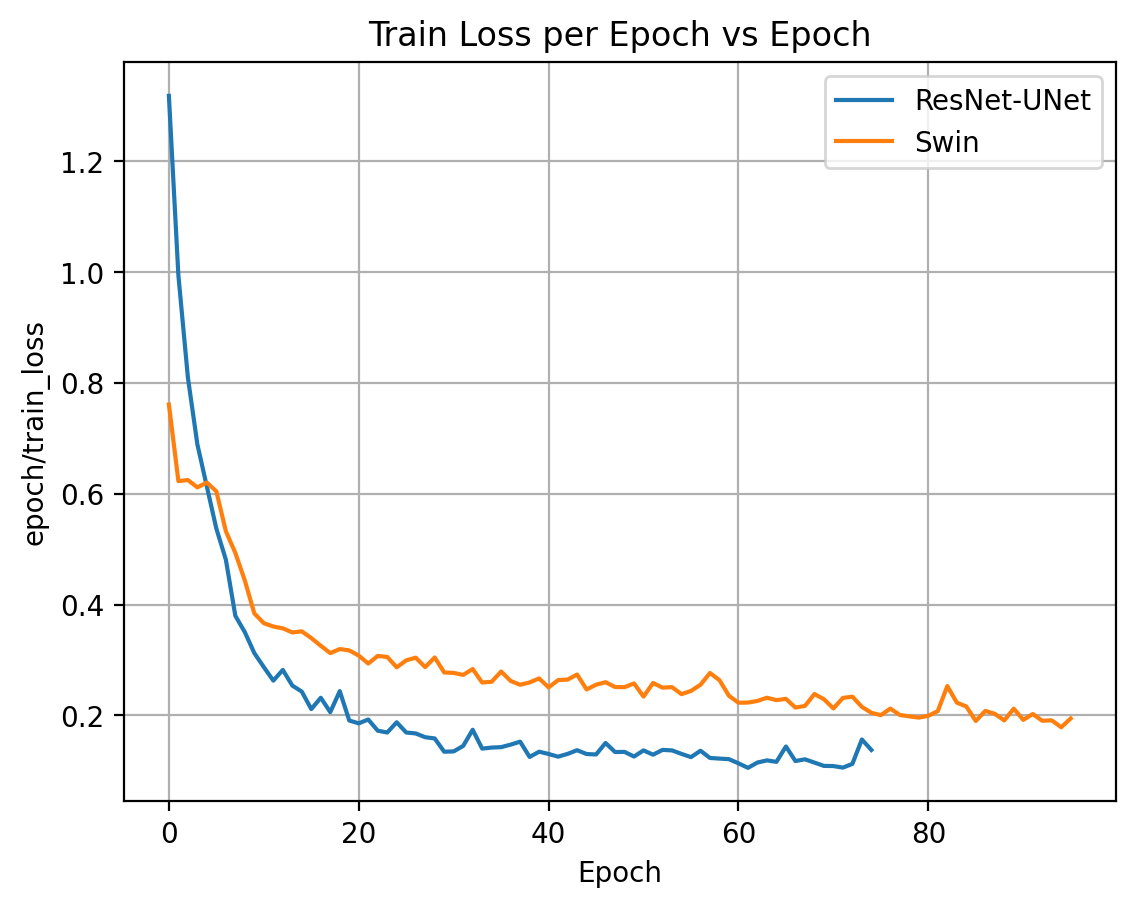
\includegraphics[width=0.6\textwidth]{Figures/chapter4/Grasping/trainloss_vs_epoch.png}
    \caption{Training loss over epochs (ResNet-UNet vs Swin).}
    \label{fig:train_loss}
\end{figure}

\begin{table}[H]
\centering
\caption{Summary of best validation results for ResNet-UNet and Swin-T models.}
\label{tab:best_val_results}
\begin{tabular}{|p{3cm}|p{2.5cm}|p{3cm}|p{3cm}|p{3cm}|}
\hline
\textbf{Model} & \textbf{Best Val Loss} & \textbf{Epoch (Best Loss)} & \textbf{Best Val Top-1 Acc} & \textbf{Epoch (Best Acc)} \\
\hline
ResNet-UNet & 0.0795 & 62 & 1.000 & 52 \\
\hline
Swin-T + Fusion & 0.1231 & 80 & 0.966 & 65 \\
\hline
\end{tabular}
\end{table}

\subsection{Qualitative Results (Inference Examples)}

To qualitatively assess the grasping models, we visualize the predicted grasp quality map and the predicted grasp orientation over representative validation samples. This visualization helps verify that the model not only achieves low numerical loss, but also produces physically meaningful grasp poses aligned with the brick geometry.

\begin{table}[H]
\centering
\caption{Qualitative comparison between labeled grasps (Ground Truth) and predicted grasps (Top-1) for three brick categories.}
\label{tab:qualitative_results}
\begin{tabular}{|l|c|c|c|}
\hline
\textbf{Sample Type} & \textbf{Ground Truth} & \textbf{ResNet-UNet} & \textbf{Swin-T} \\
\hline
I-shape & 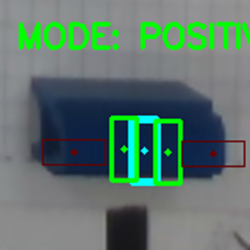
\includegraphics[width=0.2\textwidth]{Figures/chapter4/Grasping/i_gt.png} & 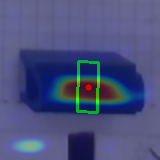
\includegraphics[width=0.2\textwidth]{Figures/chapter4/Grasping/i_resnet.png} & 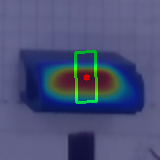
\includegraphics[width=0.2\textwidth]{Figures/chapter4/Grasping/i_swin.png} \\
\hline
L-shape & 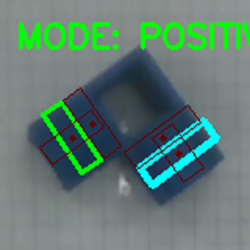
\includegraphics[width=0.2\textwidth]{Figures/chapter4/Grasping/l_gt.png} & 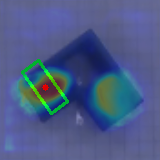
\includegraphics[width=0.2\textwidth]{Figures/chapter4/Grasping/l_resnet.png} & 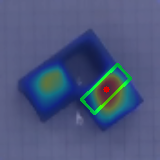
\includegraphics[width=0.2\textwidth]{Figures/chapter4/Grasping/l_swin.png} \\
\hline
T-shape & 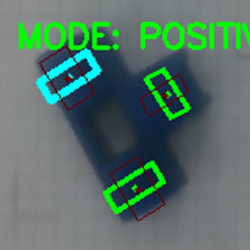
\includegraphics[width=0.2\textwidth]{Figures/chapter4/Grasping/t_gt.png} & 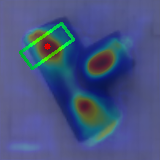
\includegraphics[width=0.2\textwidth]{Figures/chapter4/Grasping/t_resnet.png} & 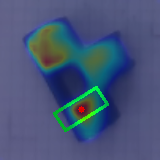
\includegraphics[width=0.2\textwidth]{Figures/chapter4/Grasping/t_swin.png} \\
\hline
\end{tabular}
\end{table}

\paragraph{Model Selection (ResNet-UNet vs Swin Transformer)}
ResNet-UNet was selected as the final deployment model for the following reasons:

\begin{itemize}
    \item \textbf{Quantitative Superiority:} It achieved lower validation loss and higher Top-1 accuracy compared to the Swin Transformer, demonstrating better agreement with supervision signals and more stable convergence.
    
    \item \textbf{Qualitative Reliability:} The model produced sharper, well-centered grasp confidence maps. in contrast, Swin Transformer outputs were often diffuse with competing peaks, increasing the risk of unreliable edge grasps.
    
    \item \textbf{Architectural Suitability:} The CNN's strong inductive bias for pixel-level localization proved advantageous for this small dataset. Transformers like Swin typically require larger datasets to learn robust attention patterns and perform effectively.
\end{itemize}